\subsection{Full SM electroweak corrections}

\label{EW:full}

\textbf{Huan-Yu Bi, Li-Hong Huang, Rui-Jun Huang, Yan-Qing Ma, Huai-Min Yu~\cite{Bi:2023bnq}.}

\noindent Ref.~\cite{Bi:2023bnq} identifies 116 integral families for the complete NLO EW corrections. The loop integrals in each family are reduced to master integrals using the {\tt Blade} package \cite{Blade}, employing {\tt FiniteFlow} \cite{Peraro:2019svx} to solve integration-by-parts (IBP) relations \cite{Chetyrkin:1981qh}, and incorporating a block-triangular form \cite{Liu:2018dmc,Guan:2019bcx} to enhance computational efficiency. Dimensional regularization is realized by choosing $\epsilon=\pm1/1000$, where $D=4-2\epsilon$. This eliminates the need for Laurent expansions in $\epsilon$ for computing the cross sections and thus reduces resource demands \cite{Liu:2022chg,Liu:2022mfb}. Master integrals are evaluated by numerically solving systems of differential equations \cite{Kotikov:1990kg,Remiddi:1997ny,Caffo:2008aw,Czakon:2008zk,Lee:2014ioa,Moriello:2019yhu,Hidding:2020ytt,Armadillo:2022ugh} in $\hat{s}$ and $\hat{t}$,  with boundary conditions computed using the {\tt AMFlow} package \cite{Liu:2022chg} implementing the auxiliary mass flow method \cite{Liu:2022mfb,Liu:2021wks,Liu:2017jxz}. The analytic continuation is performed by introducing an infinitesimal positive imaginary part to $\hat{s}$ to cross physical singularities arising in the master integrals, located at $\sqrt{\hat{s}}=2m_h$, $m_W+m_t$, $2m_t$, $2m_t+m_Z$, and $2m_t+m_h$, corresponding to intermediate particles going on-shell. The on-shell scheme for masses and fields is employed for the renormalization of the bare amplitudes, while the electromagnetic coupling $\alpha$ is renormalized in the $G_{\mu}$ scheme \cite{Denner:2019vbn}.

The cross section is obtained by integrating over the phase space,
\begin{align}\label{eq:Xsection}
\sigma^{\rm LO(NLO)} &= \frac{1}{512\pi}\int_0^1 \mathrm{d}x_{1}\int_0^1 \mathrm{d}x_{2} \int^{\hat{t}_{+}}_{\hat{t}_{-}}\mathrm{d}\hat{t} \,\times \nonumber \\
& \times \frac{1}{\hat{s}^{2}}f_{g/p}(x_{1},\mu)f_{g/p}(x_{2},\mu) M^{\rm LO(NLO)},
\end{align}
where $f_{g/p}(x,\mu)$ denotes the gluon distribution function of the proton, $\mu$ represents the factorization scale, $\hat{t}^{\pm}=m^{2}_{H}-\frac{\hat{s}}{2}(1\mp\sqrt{1-{4m^{2}_{H}}/{\hat{s}}})$, and $M^{\rm LO(NLO)}$ are given by
\begin{align}
M^{\rm LO}&=|F_{1}^{(0)}|^2+|F_{2}^{(0)}|^2 \;,\\
M^{\rm NLO}&=|F_{1}^{(0)}+F_{1}^{(1)}|^2-|F_{1}^{(1)}|^2\nonumber\\
&+|F_{2}^{(0)}+F_{2}^{(1)}|^2  -|F_{2}^{(1)}|^2,
\end{align}
where $F_i^{(0)}$ and $F_i^{(1)}$ correspond to the lowest order and the next-order terms in the $\alpha$ expansion of the form factors. The phase-space integration is carried out by optimized sampling techniques implemented through the {\tt Parni} package \cite{vanHameren:2007pt}.

The masses of the particles are set to
\begin{eqnarray}
\frac{m_h^2}{m_t^2}=\frac{12}{23}
\,,\qquad
\frac{m_Z^2}{m_t^2}=\frac{23}{83}
\,\qquad
\frac{m_W^2}{m_t^2}=\frac{14}{65}
\,,
\end{eqnarray}
with $m_t=172.69\,\textup{GeV}$ \cite{ParticleDataGroup:2022pth}. The electromagnetic coupling $\alpha=1/133.12=7.512\times 10^{-3}$ is derived from the Fermi constant $G_F=1.166378\times 10^{-5}\,\textup{GeV}^{-2}$ via
\begin{eqnarray}
\alpha=\frac{\sqrt{2}}{\pi}G_F m_W^2 \left(1-\frac{m_W^2}{m_Z^2}\right)
.
 \end{eqnarray}
The Cabibbo--Kobayashi--Maskawa (CKM) mixing matrix is set to be the unit matrix. The default PDF set for both LO and NLO calculations is NNPDF3.1 \cite{NNPDF:2017mvq}, in particular \texttt{NNPDF31\ttus nlo\ttus as\ttus 0118}. The running of the strong coupling $\alpha_s$ is taken with two-loop accuracy as provided by the {\tt LHAPDF6} library \cite{Buckley:2014ana}, including five active flavours. The default renormalization and factorization scales are $\mu=m_{hh}/2$, where $m_{hh}$ is the invariant mass of the produced Higgs boson pair.

We generate $1.8\times 10^4$ events at LO and then these events are reweighted to NLO. This enables us to calculate the $\cal{K}$ factors for the total and differential cross sections. We compute an additional 400 reweighted events per bin to reduce the statistical uncertainties for the $m_{hh}$ and $p_T$ distributions.

\begin{table}
\begin{center}
\begin{tabular}{ccccccc}
\toprule
$\mu$  & $m_{hh}/2$  & $\sqrt{p_{T}^2+m_h^2}$ & $m_h$ \\
\midrule
LO   & $19.96(6)$   & $21.11(7)$  & $25.09(8)$ \\
NLO  & $19.12(6)$   & $20.21(6)$  & $23.94(8)$ \\
${\cal K}$-factor  & $0.958(1)$   &     $0.957(1)$   &   $0.954(1)$     \\
\bottomrule
\end{tabular}
\caption{LO and NLO ${\rm EW}$-corrected integrated cross sections (in $\textup{fb}$) with $\sqrt{s}=14\,\textup{TeV}$ based on $1.8\times 10^4$ reweighted events. The uncertainties arise from statistical errors in phase space integration.}
\label{total-cs}
\end{center}
\end{table}

Table~\ref{total-cs} shows LO and NLO EW-corrected total cross sections at $\sqrt{s}=14\,\textup{TeV}$ for varying $\mu$. A difference of about $20\%$ arises for both LO and NLO cross sections from $\alpha_s$ and PDF sensitivity, which can be mitigated by higher-order QCD corrections \cite{Jones:2023uzh}. In contrast, the $\cal{K}$ factor ranges from 0.954 to 0.958 and remains stable, indicating that the EW corrections approximately factorize from the QCD corrections.

To assess the EW uncertainties, we investigate the EW corrections in the $G_{\mu}$, $\alpha_0$, and $\alpha_{m_Z}$ renormalization schemes for the electromagnetic coupling \cite{Denner:2019vbn,Sang:2024vqk}. Table~\ref{total-cs2} presents the results based on these three different schemes. We find that the scale uncertainties (or scheme uncertainties) quantified by
\begin{eqnarray}
\frac{{\rm max}(\sigma_{G_{\mu}},\sigma_{\alpha_0},\sigma_{\alpha_{m_Z}})-
      {\rm min}(\sigma_{G_{\mu}},\sigma_{\alpha_0},\sigma_{\alpha_{m_Z}})}
     {{\rm min}(\sigma_{G_{\mu}},\sigma_{\alpha_0},\sigma_{\alpha_{m_Z}})},
\end{eqnarray}
amount to $13.0\%$ at LO and are further reduced to $0.8\%$ once the EW corrections are included. These results indicate that the dominant scale uncertainties are effectively absorbed at NLO EW.

\begin{table}
\begin{center}

\begin{tabular}{ccccccc}
\toprule
 schemes  & $G_{\mu}$  & $\alpha_0$ & $\alpha_{m_Z}$ \\
\midrule
LO   & $19.96$   & $18.84$  & $21.28$ \\
NLO  & $19.12$   & $19.19$  & $19.03$ \\
${\cal K}$-factor  & $0.958$   &     $1.019$   &   $0.894$     \\
\bottomrule
\end{tabular}
\caption{LO and NLO ${\rm EW}$-corrected integrated cross sections (in $\textup{fb}$) with $\sqrt{s}=14\,\textup{TeV}$ and $\mu=m_{hh}/2$ in the $G_{\mu}$, $\alpha_0$, and $\alpha_{m_Z}$ schemes. The electromagnetic couplings are taken as $\alpha_{G_{\mu}}=1/133.12$, $\alpha_{0}=1/137.035999$, and $\alpha_{m_Z}=1/128.932$, respectively.}
\label{total-cs2}
\end{center}
\end{table}


\begin{figure}
\centering
    \subfloat[]{{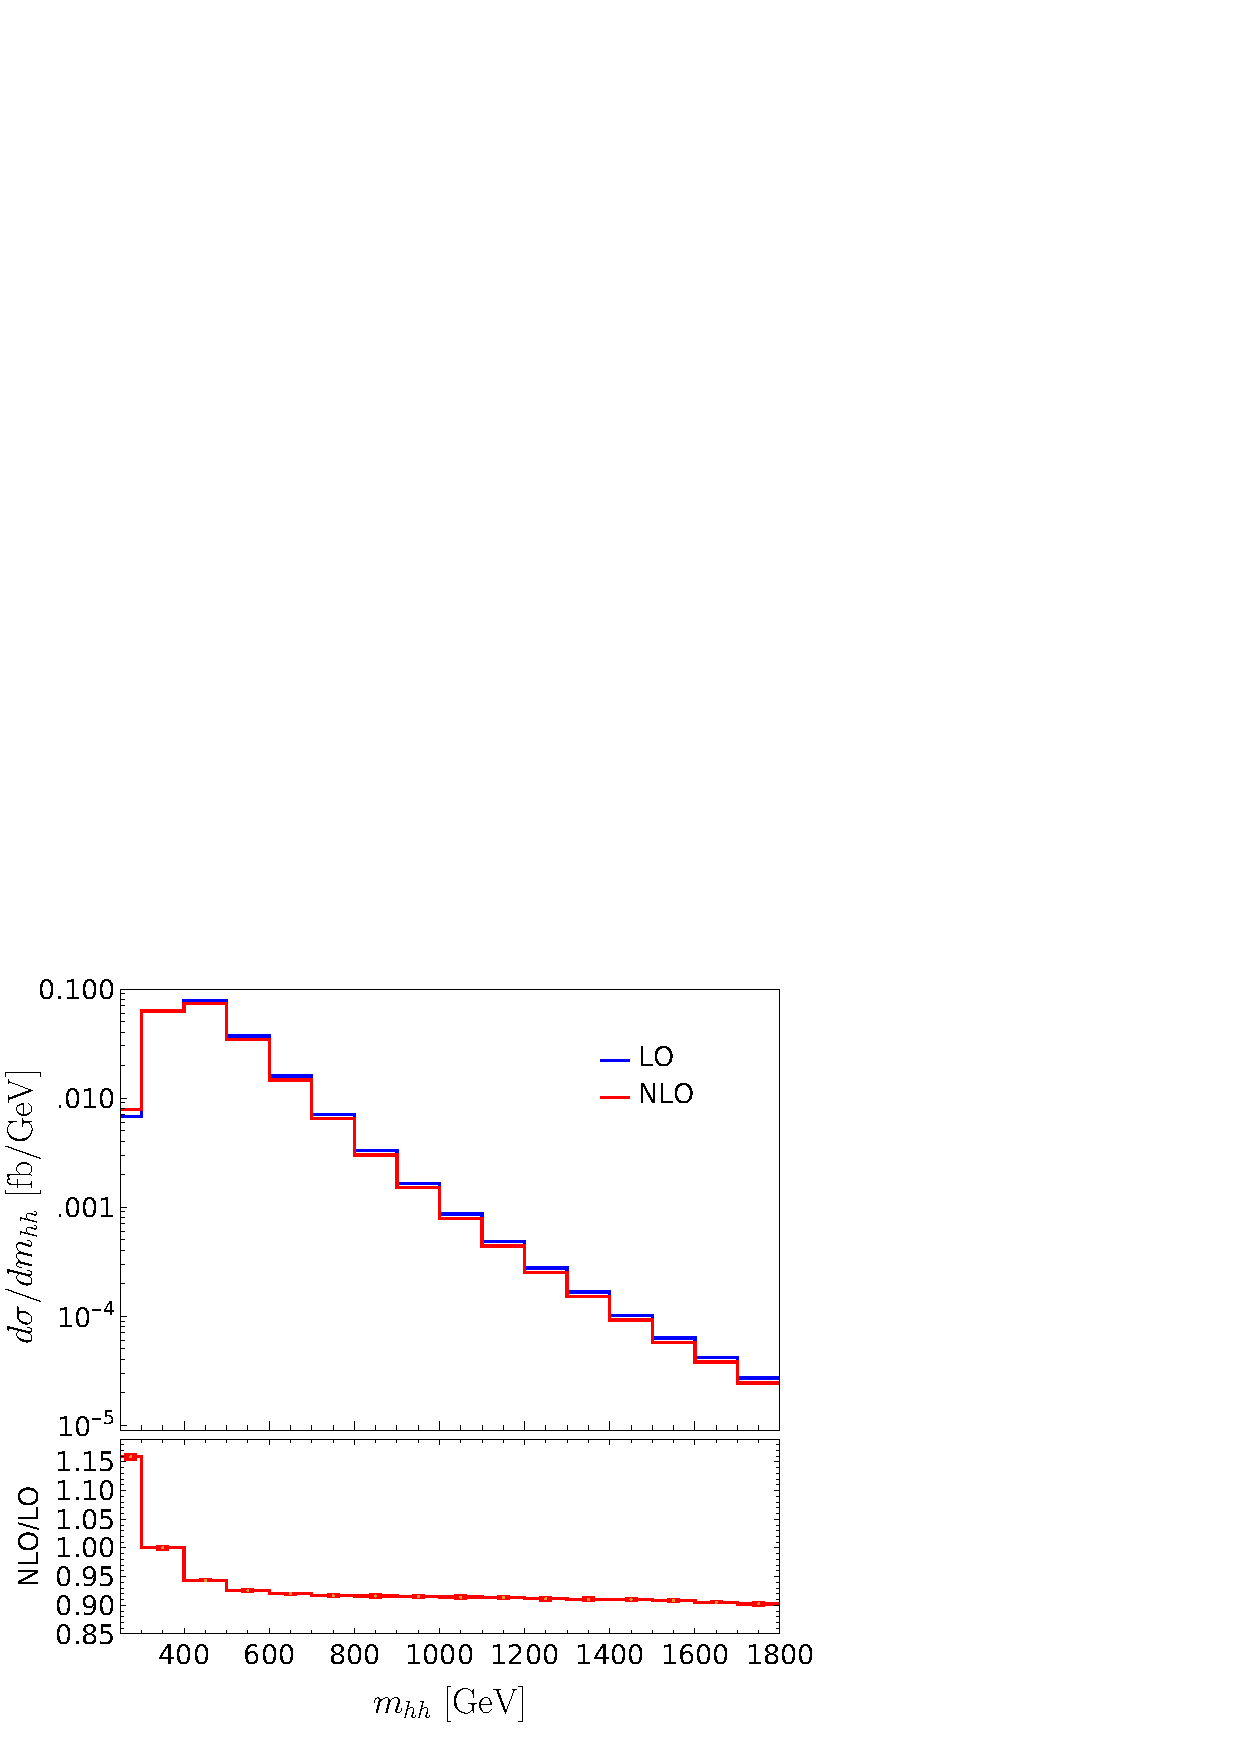
\includegraphics[width=0.47\textwidth]{NLO_EW_SM/EW_full/Images/NLO_FullEW_mhh_hlabels.pdf}}\label{mhh}}
    \subfloat[]{{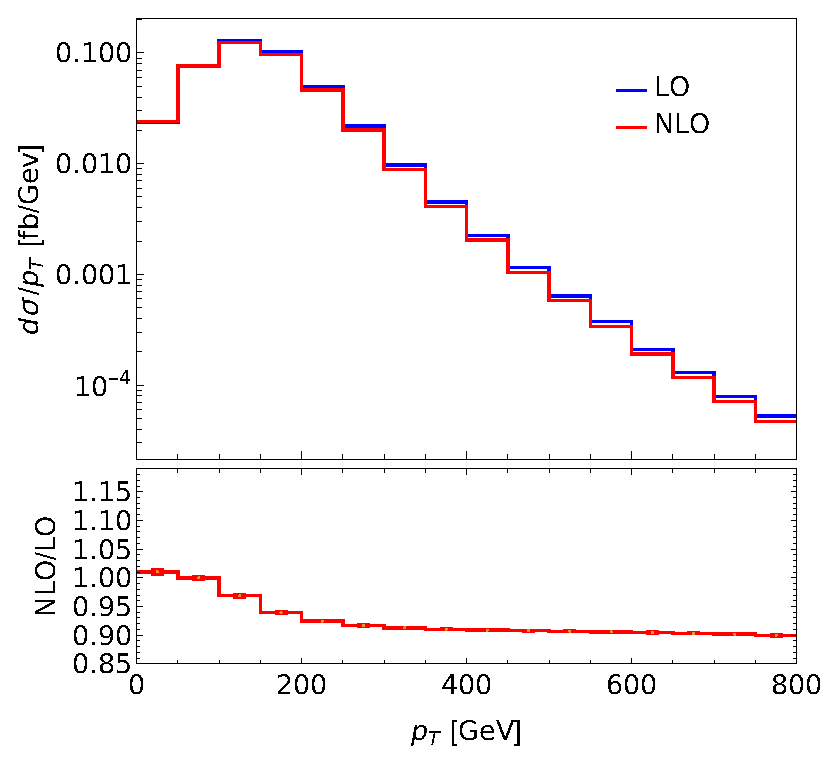
\includegraphics[width=0.47\textwidth]{NLO_EW_SM/EW_full/Images/NLO_FullEW_pth}}\label{pth}}
	\\
    \subfloat[]{{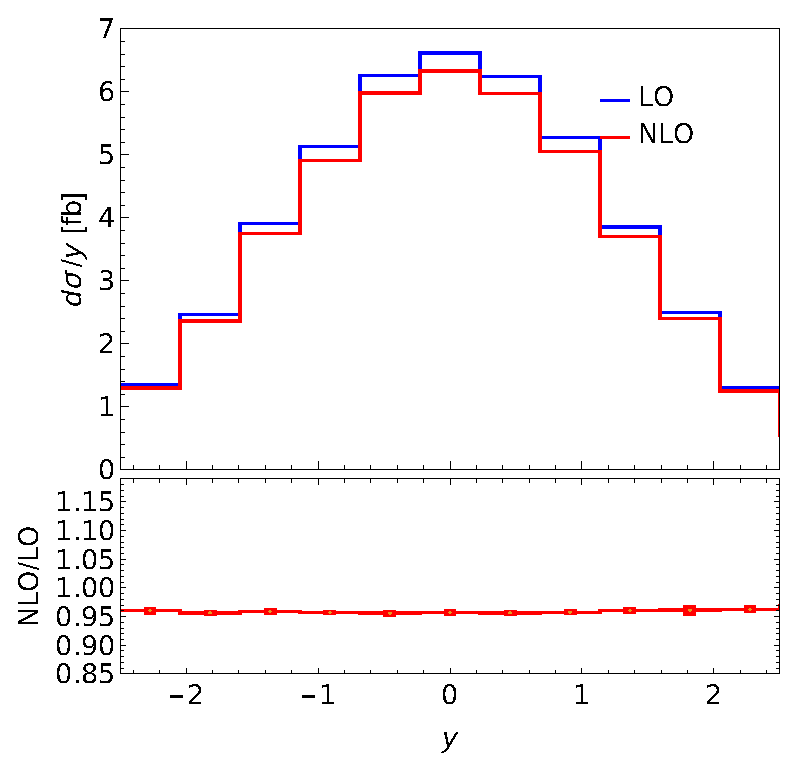
\includegraphics[width=0.47\textwidth]{NLO_EW_SM/EW_full/Images/NLO_FullEW_yh}}\label{yh}}
		\caption{Invariant mass distribution of the Higgs boson pair (a), transverse momentum distribution of one of the two Higgs bosons (b), and rapidity distribution of one of the two Higgs bosons (c), all at $\sqrt{s}=14\,\textup{TeV}$. In each panel, the upper plot shows absolute predictions and the lower panel displays the differential ${\cal K}$-factor with error bars representing statistical errors. Results shown are from Ref.~\cite{Bi:2023bnq}.}
    \label{fullEWobs}
\end{figure}


The invariant mass distribution of the Higgs boson pair $m_{hh}$ is shown in Fig.~\ref{mhh}. A significant positive correction, of approximately $+15\%$, is observed in the first bin. In fact, we find that the EW correction for phase space points near the $hh$ production threshold can exceed $+70\%$. As $m_{hh}$ increases, the $\mathcal{K}$ factor initially decreases dramatically and then becomes milder farther from the threshold. A similar pattern occurs for the $p_{T}$ distribution in Fig.~\ref{pth}, where the correction is initially positive before turning negative around $100\,\textup{GeV}$. For regions of large $m_{hh}$ or large $p_{T}$, the NLO EW correction is approximately $-10\%$. Note that, while the corrections can reach $-30\%$ for the squared matrix element at $\sqrt{\hat{s}} \approx 14\,\textup{TeV}$, the extreme suppression of the gluon luminosity at high energy makes this impact insignificant.

In Fig.~\ref{yh}, we display the rapidity distribution of one Higgs boson. The $\mathcal{K}$ factor is nearly flat, approximately $0.96$, matching that of the total cross section.
